\section{Wellen}
\begin{itemize}
    \setlength\itemsep{1pt}
    \item Ausbreitungsphänomen von E und H
    \item Ausbreitungsgeschw. kleiner $c_0$
    \item raumzeitlicher Vorgang $cos(\omega t- \beta z)$
    \item Energie- ohne Materietransport
    \item Poyntingvektor $\vec{S}=\vec{E}\times\vec{H}$ Einheit[S]$= \dfrac{W}{m^2}$\\
          {\footnotesize Falls $\vec{E}\perp\vec{H}$ und $\vec{S}\perp\vec{E}$ und $\vec{S}\perp\vec{H}$}
\end{itemize}

\subsubsection*{Wellengleichung}
\makebox[0pt][l]{
    \begin{minipage}{\columnwidth}
        \centering
        \[
            \boxed{\vec{E} = \underbrace{E_0}_{\mathclap{\text{Amplitude}}}
            \cdot \overbrace{e^{-\alpha z}}^{\mathclap{\text{Dämpfung}}}
            \cdot \underbrace{cos(\omega t \overbrace{-}^{\mathclap{\text{positive z-Richtung}}} \beta z)}_\text{zeitraum Abhängigkeit}}
        \]
        {\footnotesize Analog für H-Feld}
    \end{minipage}
}

\subsubsection*{Fortpflanzungskonstante $\gamma$}
\[\boxed{\underline{\gamma}=\alpha+j\beta}\]

$\alpha$ : Dämpfungskonst. [Np/m]

$\beta$ : Phasenkonst. [rad/m]

$v$ : Phasengeschw. [m/s]

\subsection{Ausbreitung}
\subsubsection{Allgemein}
\begin{align*}
     & \alpha = \omega \cdot \sqrt{\dfrac{\mu \varepsilon}{2}\cdot \left(\sqrt{1+\dfrac{\sigma^2}{\omega^2\cdot\varepsilon^2}}{\color{red}{-}}1\right)}   \\
     & \beta  = \omega \cdot \sqrt{\dfrac{\mu \varepsilon}{2}\cdot \left(\sqrt{1+\dfrac{\sigma^2}{\omega^2\cdot\varepsilon^2}}{\color{green}{+}}1\right)} \\
     & \underline{Z}_F = \sqrt{\dfrac{j\omega\mu}{\sigma+j\omega\varepsilon}}                                                                             \\
     & E_2 = E_1 \cdot e^{-\alpha z}                                                                                                                      \\
     & H = \dfrac{E}{Z_F}
\end{align*}

\subsubsection{Im leeren Raum(Vakuum)}
\begin{align*}
     & \alpha = 0                                                                                 \\
     & \beta = \dfrac{\omega}{c_0}                                                                \\
     & \boxed{\underline{Z}_{F0} = \sqrt{\dfrac{\mu_0}{\varepsilon_0}}\text{ }=\text{ }377\Omega} \\
     & \lambda = \dfrac{c_0}{f}                                                                   \\
     & v = c_0
\end{align*}

\subsubsection{Im Dielektrika mit geringem Verlust}
verlustlos: $\sigma =0$
\begin{align*}
     & \alpha = 0                                                                                                       \\
     & \beta = \dfrac{\omega}{c_0}\cdot\sqrt{\mu_r\varepsilon_r}=\omega\cdot\sqrt{\mu\varepsilon}=\dfrac{2\pi}{\lambda} \\
     & \underline{Z}_F = \sqrt{\dfrac{\mu}{\varepsilon}}                                                                \\
     & \lambda = \dfrac{c_0}{f}\cdot\dfrac{1}{\sqrt{\mu_r\varepsilon_r}}=\dfrac{2\pi}{\beta}                            \\
     & v = \dfrac{c_0}{\sqrt{\mu_r\varepsilon_r}}
\end{align*}

\subsubsection{Im Dielektrika mit geringem Verlust}
geringer Verlust: $0 < \sigma \ll\omega\varepsilon$
\begin{align*}
     & \alpha = \dfrac{1}{2}\cdot\sigma\cdot\sqrt{\dfrac{\mu}{\varepsilon}}                                                      \\
     & \beta = \omega\cdot\sqrt{\mu\varepsilon}\cdot\left(1+\dfrac{1}{8}\cdot\dfrac{\sigma^2}{\omega^2\cdot\varepsilon^2}\right) \\
     & \underline{Z}_F = \sqrt{\dfrac{\mu}{\varepsilon}}                                                                         \\
     & \lambda = \dfrac{c_0}{f}\cdot\dfrac{1}{\sqrt{\mu_r\varepsilon_r}}=\dfrac{2\pi}{\beta}                                     \\
     & v = \dfrac{c_0}{\sqrt{\mu_r\varepsilon_r}}
\end{align*}

\subsubsection{Im guten Leiter}
geringer Verlust: $\sigma \gg\omega\varepsilon$
\begin{align*}
     & \alpha = \dfrac{1}{\delta}= \beta                                                                                                           \\
     & \underline{Z}_F = \sqrt{\dfrac{j\omega\mu}{\sigma}} = \sqrt{\dfrac{\omega\mu}{2\sigma}}\cdot\left(1+j\right)=\dfrac{1+j}{\sigma\cdot\delta} \\
     & \lambda = \dfrac{2\pi}{\beta} = 2\pi \sqrt{\dfrac{2}{\omega\mu\sigma}}=2\pi\delta                                                           \\
\end{align*}

\subsection{Übergang}
\subsubsection{Zwischen Dielektrika mit geringem Verlust}
%bitte ergänzen
\makebox[0pt][l]{
    \begin{minipage}{\columnwidth}
        \centering
        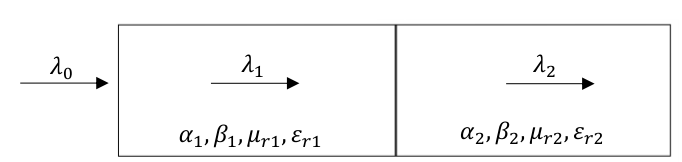
\includegraphics[width=.8\columnwidth]{Figures/UebergangzweiDielektrika.png}
        \label{fig:UebergangzweiDielektrika}
    \end{minipage}
}

\begin{align}
    \lambda_1 = \dfrac{\lambda_0}{\sqrt{\mu_{r1}\varepsilon_{r1}}}        &  & \lambda_2 = \dfrac{\lambda_0}{\sqrt{\mu_{r2}\varepsilon_{r2}}}                           \\
                                                                          &  & = \dfrac{\lambda_1\cdot\sqrt{\mu_{r1}\varepsilon_{r1}}}{\sqrt{\mu_{r2}\varepsilon_{r2}}} \\
    \beta_1 = \dfrac{2\pi}{\lambda_0}\cdot\sqrt{\mu_{r1}\varepsilon_{r1}} &  & \beta_2 = \dfrac{2\pi}{\lambda_0}\cdot\sqrt{\mu_{r2}\varepsilon_{r2}}                    \\
    Z_{F1} = \dfrac{Z_{F0}}{\sqrt{\mu_{r1}\varepsilon_{r1}}}              &  & Z_{F2} = \dfrac{Z_{F0}}{\sqrt{\mu_{r2}\varepsilon_{r2}}}
\end{align}
\subsection{Energie und Poyntingvektor (Energieflussdichte)}
\begin{align*}
     & \vec{S} = \vec{E}\times\vec{H} \text{ in } [W/m^2]                                   \\
     & S = 1/2 \cdot E \cdot H = 1/2 \cdot \dfrac{E^2}{Z_{F0}} = 1/2 \cdot H^2 \cdot Z_{F0} \\
     & \underline{S}_{Mittel} = 1/2 \cdot Re\{\vec{E}\times\vec{H}^*\}                      \\
     & S = \dfrac{P}{A}                                                                     \\
\end{align*}
\subsubsection{Leistung nach Dämpfung}
\begin{align*}
     & P_1 = P_0 \cdot e^{-2\alpha z}                              \\
     & P = \dfrac{\hat{U}^2}{2 Z_L} \text{vom Kabel transportiert}
\end{align*}
\subsection{dÀlembertsche Gleichung (allg.)}

\begin{align*}
    \Delta \vec{E}-\kappa \mu \frac{\partial \vec{E}}{\partial t}-\varepsilon \mu \frac{\partial^{2} \vec{E}}{\partial t^{2}} & = \operatorname{grad} \frac{\rho}{\varepsilon} \\
    \Delta \vec{H}-\kappa \mu \frac{\partial \vec{H}}{\partial t}-\varepsilon \mu \frac{\partial^{2} \vec{H}}{\partial t^{2}} & = 0
\end{align*}

Isolator, ideales Dielektrikum, Nichtleiter $\kappa = 0$
\begin{align*}
    \Delta \vec{E} & =\varepsilon \mu \frac{\partial^{2} \vec{E}}{\partial t^{2}}+\operatorname{grad} \frac{\rho}{\varepsilon} \\
    \Delta \vec{H} & =\varepsilon \mu \frac{\partial^{2} \vec{H}}{\partial t^{2}}
\end{align*}

sehr gute Leiter
\begin{align*}
    \Delta \vec{E} & =\kappa \mu \frac{\partial \vec{E}}{\partial t}+\operatorname{grad} \frac{\rho}{\varepsilon} \\
    \Delta \vec{H} & =\kappa \mu \frac{\partial \vec{H}}{\partial t}
\end{align*}

\subsection{Helmholtz-Gleichungen (Frequenzbereich)}
\begin{align*}
    \Delta \underline{\vec{E}}-\left(\kappa \mu \cdot \mathrm{j} \omega-\varepsilon \mu \cdot \omega^{2}\right) \cdot \underline{\vec{E}} & = \operatorname{grad} \frac{\rho}{\varepsilon} \\
    \Delta \underline{\vec{H}}-\left(\kappa \mu \cdot \mathrm{j} \omega-\varepsilon \mu \cdot \omega^{2}\right) \cdot \underline{\vec{H}} & = 0
\end{align*}

\subsubsection{Zeitbereich}
\begin{align*}
    \Delta \vec{E}-\varepsilon \mu \frac{\partial^{2} \vec{E}}{\partial t^{2}} & =0 \\
    \Delta \vec{H}-\varepsilon \mu \frac{\partial^{2} \vec{H}}{\partial t^{2}} & =0
\end{align*}

\subsubsection{Frequenzbereich (harmonisch)}
\begin{align*}
    \Delta \underline{\vec{E}}+\varepsilon \mu \omega^{2} \cdot \underline{\vec{E}} & =0 \\
    \Delta \underline{\vec{H}}+\varepsilon \mu \omega^{2} \cdot \underline{\vec{H}} & =0
\end{align*}

%%%%%%%%%%%%%%%%%

\subsection{Wellenzahl}
Im Vakuum: $k_{0}=\frac{\omega}{c_{0}}$
\begin{align*}
    k & = \frac{\omega}{v_{p h}} = \frac{2 \pi f}{v_{p h}} = |\vec{k}|                                                              \\
      & = \frac{\omega \cdot n}{c_{0}} = n \cdot k_{0}=\frac{1}{\sqrt{\mu_{r} \cdot \varepsilon_{r}}} \cdot k_{0}=k_{r} \cdot k_{0}
\end{align*}

\subsection{Wellenlänge}
\begin{align*}
    \lambda   & = \dfrac{\lambda_0}{\sqrt{\mu_r \cdot \varepsilon_r}} = \dfrac{2 \pi}{k} = \dfrac{v_{ph}}{f} = [m] \\
              & = \dfrac{\lambda_0}{n} = \dfrac{2 \pi}{n \cdot k_0}                                                \\
    \lambda_0 & = \dfrac{c_0}{f} = \dfrac{2\pi}{k_0}
\end{align*}

\subsection{Phasengeschwindigkeit}
\[
    \dfrac{d z}{d t} = \upsilon_{ph} = c = \dfrac{\omega}{k} = \frac{1}{\sqrt{ \mu_r \mu_0 \varepsilon_r \varepsilon_0}} \qquad \upsilon_{ph,\textnormal{Medium} \leq c_0}
\]
%\subsection{Ausbreitung im leeren Raum(Vakuum)}
%\[
%    \text{penis}
%\]

\subsubsection{Gruppengeschwindigkeit}
\[
    \upsilon_{g} = \dfrac{d \omega}{d k} = \dfrac{\textnormal{Wegstück der Wellengruppe}}{\textnormal{Laufzeit der Wellengruppe}}
\]

% \subsection{Feldwellenwiderstand}
% allgemein, idealen Dielektrikum\\
% freier Raum
% \begin{align*}
%     \underline{Z}_F    & = \dfrac{\underline{E}_{\textnormal{transversal}}}{\underline{H}_{\textnormal{transversal}}} = \sqrt{\dfrac{\mu}{\varepsilon}} \\
%     \underline{Z}_{F0} & = \sqrt{\dfrac{\mu_0}{\varepsilon_0}} \approx 120\pi \Omega \approx 377 \Omega
% \end{align*}

\subsection{Polarisation}
\begin{tabularx}{0.45\textwidth}{>{\hsize=.3\hsize}X|>{\hsize=.7\hsize}X}
    Lineare     & wenn der Endpunkt des E–Vektors eine Linie     \\
    \hline
    Elliptische & Endpunkt des E-Vektors eine Ellipse beschreibt
\end{tabularx}
